\documentclass[a4paper]{article}
\usepackage[utf8]{inputenc}
\usepackage[russian,english]{babel}
\usepackage[T2A]{fontenc}
\usepackage[left=10mm, top=20mm, right=18mm, bottom=15mm, footskip=10mm]{geometry}
\usepackage{indentfirst}
\usepackage{amsmath,amssymb}
\usepackage[italicdiff]{physics}
\usepackage{graphicx}
\graphicspath{{images/}}
\DeclareGraphicsExtensions{.pdf,.png,.jpg}
\usepackage{wrapfig}
\usepackage{float}
\usepackage{subcaption}
\usepackage{enumitem}
\usepackage{caption}
\captionsetup[figure]{name=Рисунок}
\captionsetup[table]{name=Таблица}

\title{\underline{Отчет о выполненой лабораторной работе 3.6.1}}
\author{Воронин Денис, Дрожжин Никита Б04-407}

\begin{document}

\maketitle

\begin{center}
\textbf{\Large СПЕКТРАЛЬНЫЙ АНАЛИЗ ЭЛЕКТРИЧЕСКИХ СИГНАЛОВ}
\end{center}


\indent \textbf{Цель работы:} изучить спектры сигналов различной формы и влияние параметров сигнала
на вид соответствующих спектров; проверить справедливость соотношений неопределённостей; познакомиться с работой спектральных фильтров на примере RC-цепочки

\indent \textbf{В работе используются:} генератор сигналов произвольной формы, цифровой осциллограф с функцией быстрого преобразования Фурье или цифровой USB-осциллограф, подключённый к персональному компьютеру.

\section{Теоретическое введение}

\subsection*{Разложение сложных сигналов на периодические колебания}
Представление периодического сигнала в виде суммы гармонических сигналов называется разложением в ряд Фурье.
	
	Пусть заданная функция $f(t)$ периодически повторяется с частотой $\Omega_{1}=\dfrac{2\pi}{T},$ где $T$ - период повторения. Ее разложение в ряд Фурье имеет вид
\begin{equation}
    f(t)=\dfrac{a_{0}}{2}+ \sum\limits_{n=1}^\infty [a_{n}\cos(n \Omega_{1}t)+b_{n}\sin(n \Omega_{1} t) ]
\label{eq1}
\end{equation}
		Здесь $\dfrac{a_{0}}{2}$ - среднее значение функции $f(t)$,
	
\begin{equation}
     a_{n}=\dfrac{2}{T}\int\limits_{t_{1}}^{t_{1}+T}f(t)\cos(n \Omega_{1} t)dt, 
     \label{eq2}
\end{equation}
\begin{equation}
    b_{n}=\dfrac{2}{T}\int\limits_{t_{1}}^{t_{1}+T}f(t)\sin(n \Omega_{1} t)dt.
    \label{eq3}
\end{equation}
  

	
	
	Рассмотрим периодические функции, которые исследуются в нашей
	работе.
	
	\begin{enumerate}
		
	\item 	\textbf{Периодическая последовательность прямоугольных импульсов} (рис. 1) с амплитудой $V_{0}$, длительностью $\tau$, частотой повторения $\Omega_{1}=\dfrac{2\pi}{T},$ где $T$ - период повторения импульсов. Найдем коэффициенты разложения ряда Фурье:
	
	$$\dfrac{a_{0}}{2}=V_{0}\dfrac{\tau}{T},$$

 \begin{equation}
     a_{n}=\dfrac{2}{T}\int\limits_{-\frac{\tau}{2}}^{\frac{\tau}{2}}V_{0}\cos(n \Omega_{1} t)dt=2V_{0}\dfrac{\tau}{T}\dfrac{\sin(n \Omega_{1} \frac{\tau}{2})}{n\Omega_{1}\frac{\tau}{2}} \sim \dfrac{\sin x}{x}.
    \label{eq4}
 \end{equation}

	
	Поскольку наша функция четная, все коэффициенты синусоидальных гармоник $b_{n}=0$. Спектр $a_{n}$ последовательности прямоугольных импульсов представлен на рис. 2 (изображен случай, когда $T$ кратно $\tau$).
		
		
		\begin{figure}[h]
			\begin{minipage}[h]{0.5\linewidth}
				\center{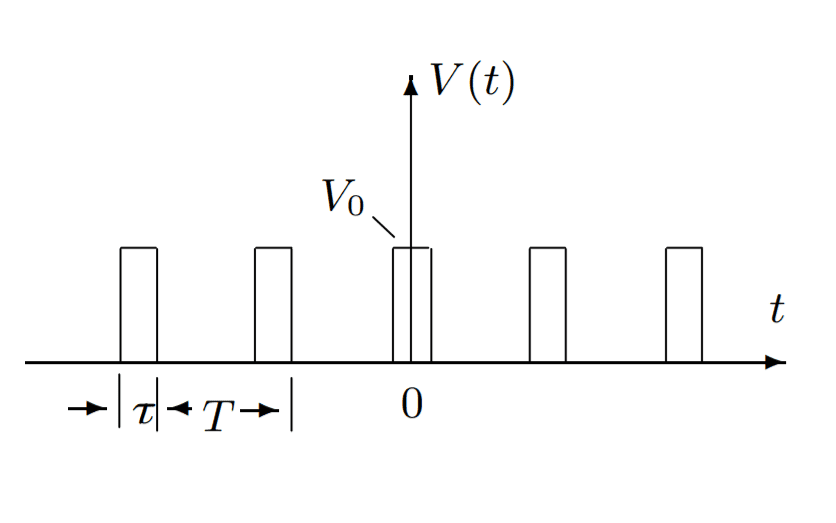
\includegraphics[width=0.9\linewidth]{sp1.png}}
				\caption{Прямоугольные импульсы}
			\end{minipage}
			\begin{minipage}[h]{0.5\linewidth}
				\center{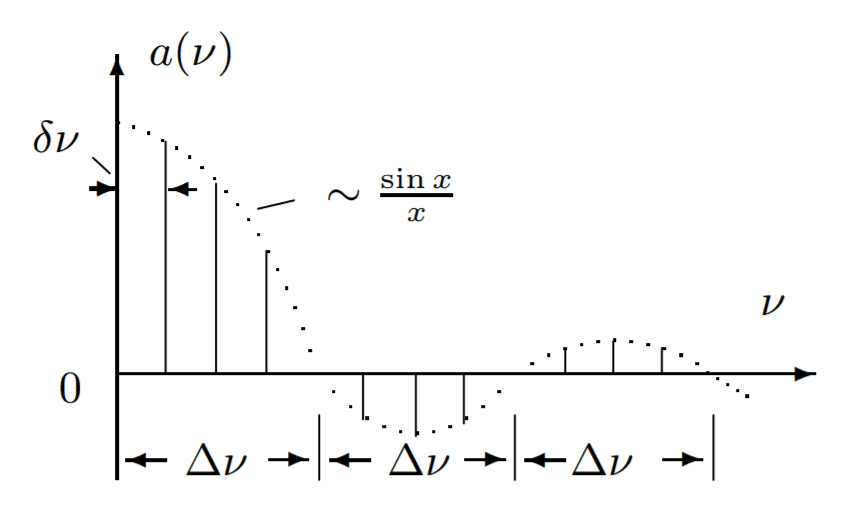
\includegraphics[width=0.9\linewidth]{sp2.png}}
				\caption{Спектр последовательности прямоугольных импульсов}
			\end{minipage}
		\end{figure}
	
	Назовем \textit{шириной спектра} $\Delta \omega$ расстояние от главного максимума ($\omega =0$) до первого нуля огибающей, возникающего при $n=\dfrac{2\pi}{\tau \Omega_{1}}$. При этом 

	$$\Delta \omega \tau \backsimeq 2 \pi $$
	
	 или 
	
\begin{equation}\label{neopr}
	\Delta \nu \Delta t \backsimeq 1
\end{equation}
		
	Полученное соотношение взаимной связи интервалов $\Delta \nu$ и $\Delta t$ является
	частным случаем соотношения неопределенности в квантовой механике.
	
	\item \textbf{Периодическая последовательность цугов} гармонического колебания $V_{0}\cos(\omega_{0}t)$ с длительностью цуга $\tau$ и периодом повторения $T$ (рис. 3).
	
	Функция $f(t)$ снова является четной относительно $t=0$. Коэффициент при $n$-й гармонике равен
\begin{equation}
    a_{n}=\dfrac{2}{T}\int\limits_{-\frac{\tau}{2}}^{\frac{\tau}{2}}V_{0}\cos(\omega_{0}t)\cos(n \Omega_{1} t)dt=V_{0}\dfrac{\tau}{T} \bigg(\dfrac{\sin[(\omega_{0}-n\Omega_{1})\frac{\tau}{2}]}{(\omega_{0}-n\Omega_{1})\frac{\tau}{2}}+\dfrac{\sin[(\omega_{0}+n\Omega_{1})\frac{\tau}{2}]}{(\omega_{0}+n\Omega_{1})\frac{\tau}{2}} \bigg)
\label{eq6}
\end{equation}
	
	Зависимость для случая, когда $\frac{T}{\tau}$ равно целому числу, представлена на рис. 4. Сравнивая спектр последовательности прямоугольных импульсов и цугов мы видим, что они аналогичны, но их максимумы сдвинуты по частоте на величину $\omega_{0}$.
	
	\begin{figure}[h]
		\begin{minipage}[h]{0.5\linewidth}
			\center{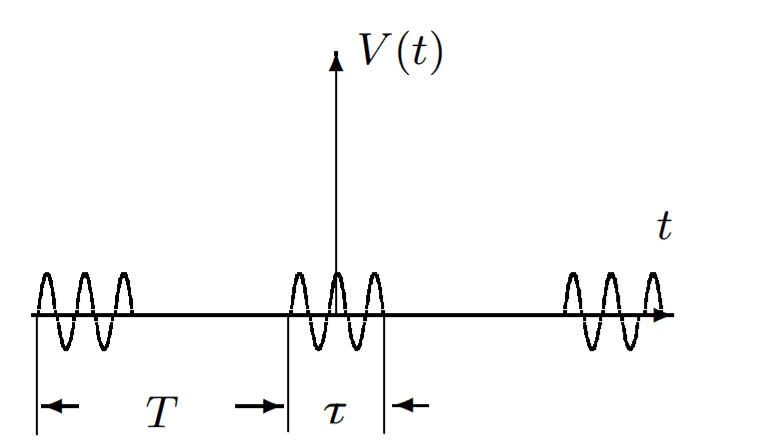
\includegraphics[width=0.9\linewidth]{sp3.png}}
			\caption{Последовательность цугов}
		\end{minipage}
		\begin{minipage}[h]{0.5\linewidth}
			\center{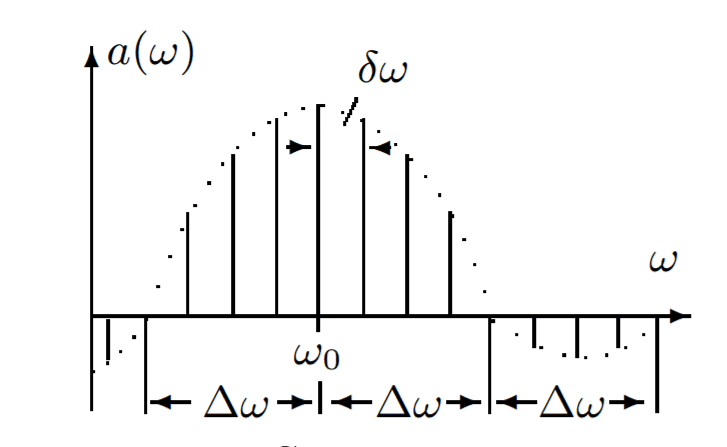
\includegraphics[width=0.9\linewidth]{sp4.png}}
			\caption{Спектр последовательности цугов}
		\end{minipage}
	\end{figure}

	\item \textbf{Амплитудно-модулированные колебания.} Рассмотрим гармонические колебания высокой частоты $\omega_{0}$ , амплитуда которых медленно меняется по гармоническому закону с частотой $\Omega$ ($\Omega \ll \omega_{0})$) (рис. 5):
\begin{equation}
    f(t)=A_{0}[1+m\cos\Omega t]\cos \omega_{0}t
\label{eq7}
\end{equation}	

	Коэффициент $m$ называют \textbf{глубиной модуляции}. При $m<1$ амплитуда колебаний меняется от минимальной $A_{min}=A_{0}(1-m)$ до максимальной $A_{max}=A_{0}(1+m).$ Глубина модуляции может быть представлена в виде
	
\begin{equation}\label{m}
	 m=\dfrac{A_{max}-A_{min}}{A_{max}+A_{min}}
\end{equation}
	
	Простым тригонометрическим преобразованием можно найти спектр амплитудно - модулированных колебаний:
	\\
\begin{equation}\label{a}
	f(t)=A_{0}\cos(\omega_{0} t)+\dfrac{A_{0}m}{2}\cos(\omega_{0}+\Omega)t+\dfrac{A_{0}m}{2}\cos(\omega_{0}-\Omega)t.
\end{equation}
		
		\begin{figure}[h]
			\begin{minipage}[h]{0.5\linewidth}
				\center{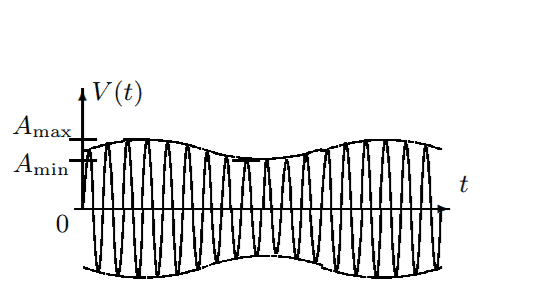
\includegraphics[width=0.9\linewidth]{sp5.png}}
				\caption{Модулированные гармонические колебания}
			\end{minipage}
			\begin{minipage}[h]{0.5\linewidth}
				\center{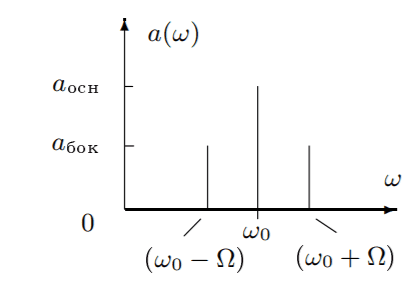
\includegraphics[width=0.9\linewidth]{sp6.png}}
				\caption{Спектр модулированных гармонических колебаний}
			\end{minipage}
		\end{figure}
		
		Спектр таких колебаний содержит три составляющих  основную
		компоненту и две боковых (рис. 6). Первое слагаемое в правой части представляет собой исходное немодулированное колебание
		с основной (несущей) частотой $\omega_{0}$ и амплитудой $a_{осн} = A_{0}$ . Второе и третье слагаемые соответствуют новым гармоническим колебаниям с частотами $\omega_{0} + \Omega$ и $\omega_{0} - \Omega$. Амплитуды этих двух колебаний одинаковы и составляют $\dfrac{m}{2}$ от амплитуды немодулированного колебания:
		$a_{бок} = \dfrac{A_{0}m}{2}$. Начальные фазы всех трех колебаний одинаковы.
	\end{enumerate}

\section{Ход работы}

\subsection{А. Исследование спектра периодической последовательности  
прямоугольных импульсов и проверка соотношений неопределённостей }



\textbf{1.} Следуя техническому описанию генератора (п. А), мы настраиваем генерацию прямоугольных импульсов. Рекомендуемые параметры: частота повторения \( v_{\text{повт}} = 1 \) кГц (период \( T = 1/v_{\text{повт}} = 1 \) мс), и длительность импульса \( \tau = T/20 = 50 \) мкс.

\textbf{2.} Мы получаем устойчивую картину сигнала на экране осциллографа (см. техническое описание осциллографа, п. I).

\textbf{3.} Следуя техническому описанию осциллографа (п. II), мы получаем на его экране спектр (преобразование Фурье) сигнала.

Масштаб по горизонтальной оси мы устанавливаем меньше или порядка ожидаемой ширины спектра \( \Delta v \) (ширина спектра оценивается из соотношения неопределенностей).

Масштаб по вертикальным осям мы подбираем так, чтобы спектральные линии не выходили за пределы экрана (кроме, может быть, «нулевой» гармоники \( v = 0 \) Гц — она отвечает за уровень постоянного смещения сигнала, и ее высота может оказаться значительно выше остальных).

Центр картины при предварительной настройке мы устанавливаем на 0 Гц, а затем после подбора масштабов смещаем его так, чтобы спектр занимал весь экран, начиная от левого края.

\textbf{4.}Изменяя на генераторе параметры сигнала, мы наблюдаем, как изменяется спектр. 
В лабораторном журнале мы записываем, что происходит со спектром:
\begin{enumerate}
    \item[а)] при изменении $\nu_{\text{повт}}$ при фиксированном $\tau$;
    \item[б)] при изменении $\tau$ при фиксированном $\nu_{\text{повт}}$.
\end{enumerate}
а) увеличивается расстояние между компонентами спектра\par
б)уменьшается ширина спектра


\begin{figure}[ht]
    \centering
    \begin{minipage}{0.48\textwidth}
        \centering
        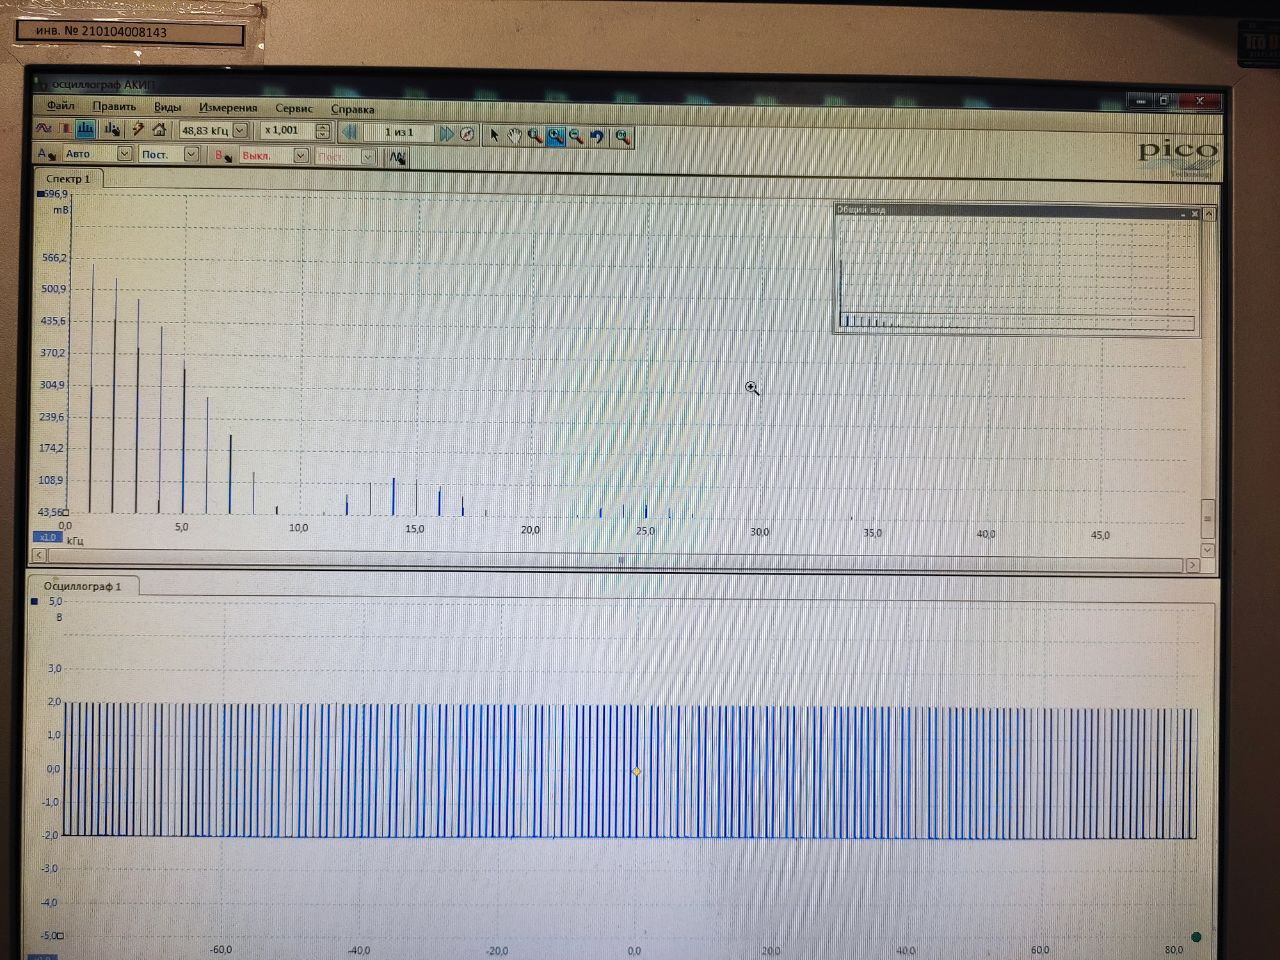
\includegraphics[width=10 cm]{50_1k.jpg}
        \caption{при изменении $\nu_{\text{повт} = 1000 Hz}$ при фиксированном $\tau = 50 nsec$}
        \label{fig:image1}
    \end{minipage}\hfill
    \begin{minipage}{0.48\textwidth}
        \centering
        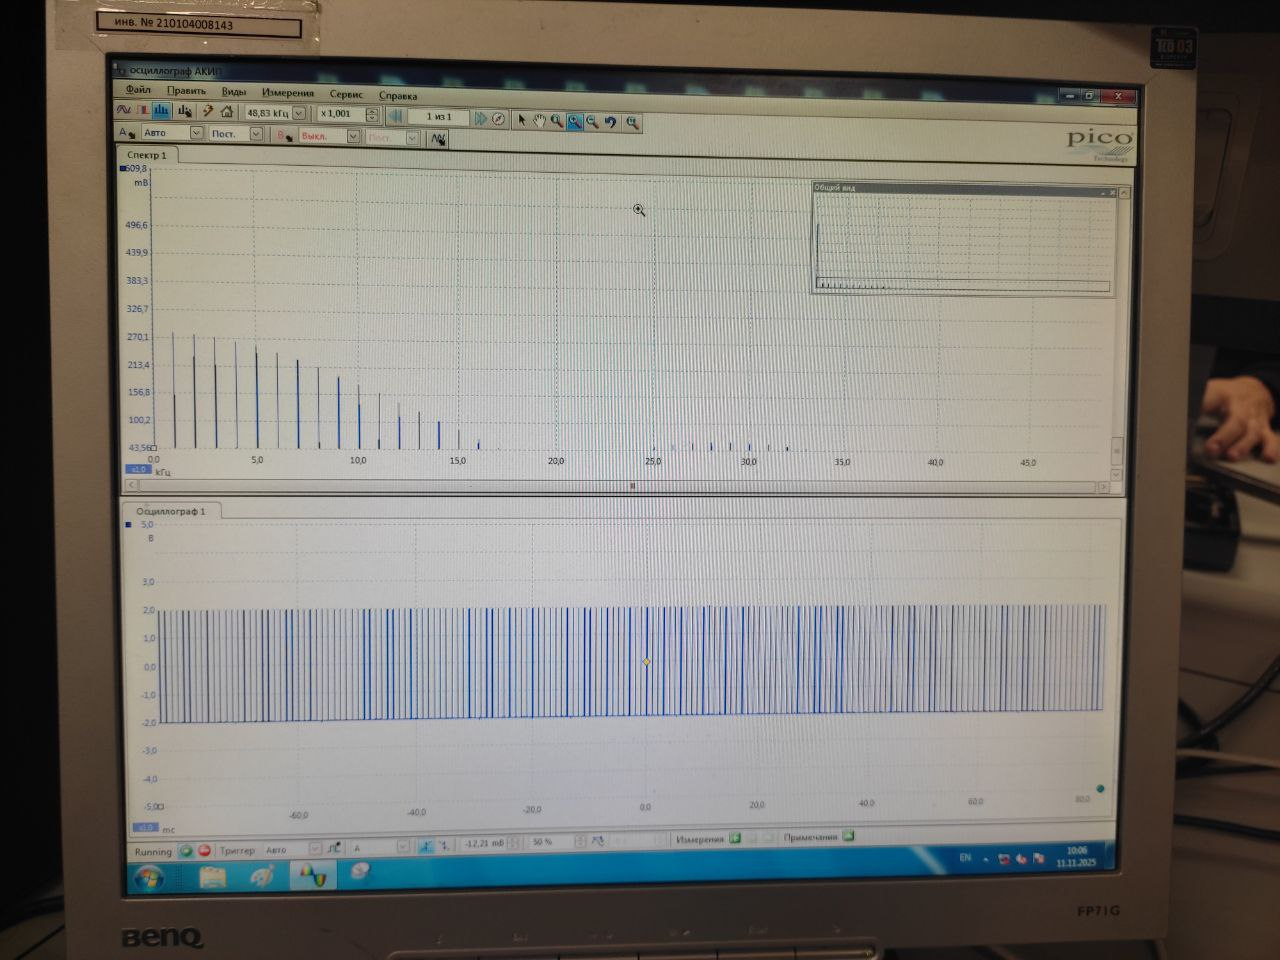
\includegraphics[width=10 cm]{50_9.jpg}
        \caption{при изменении $\nu_{\text{повт} = 9000 Hz}$ при фиксированном $\tau = 50 nsec$}
        \label{fig:image2}
    \end{minipage}
\end{figure}

\begin{figure}[ht]
    \centering
    \begin{minipage}{0.48\textwidth}
        \centering
        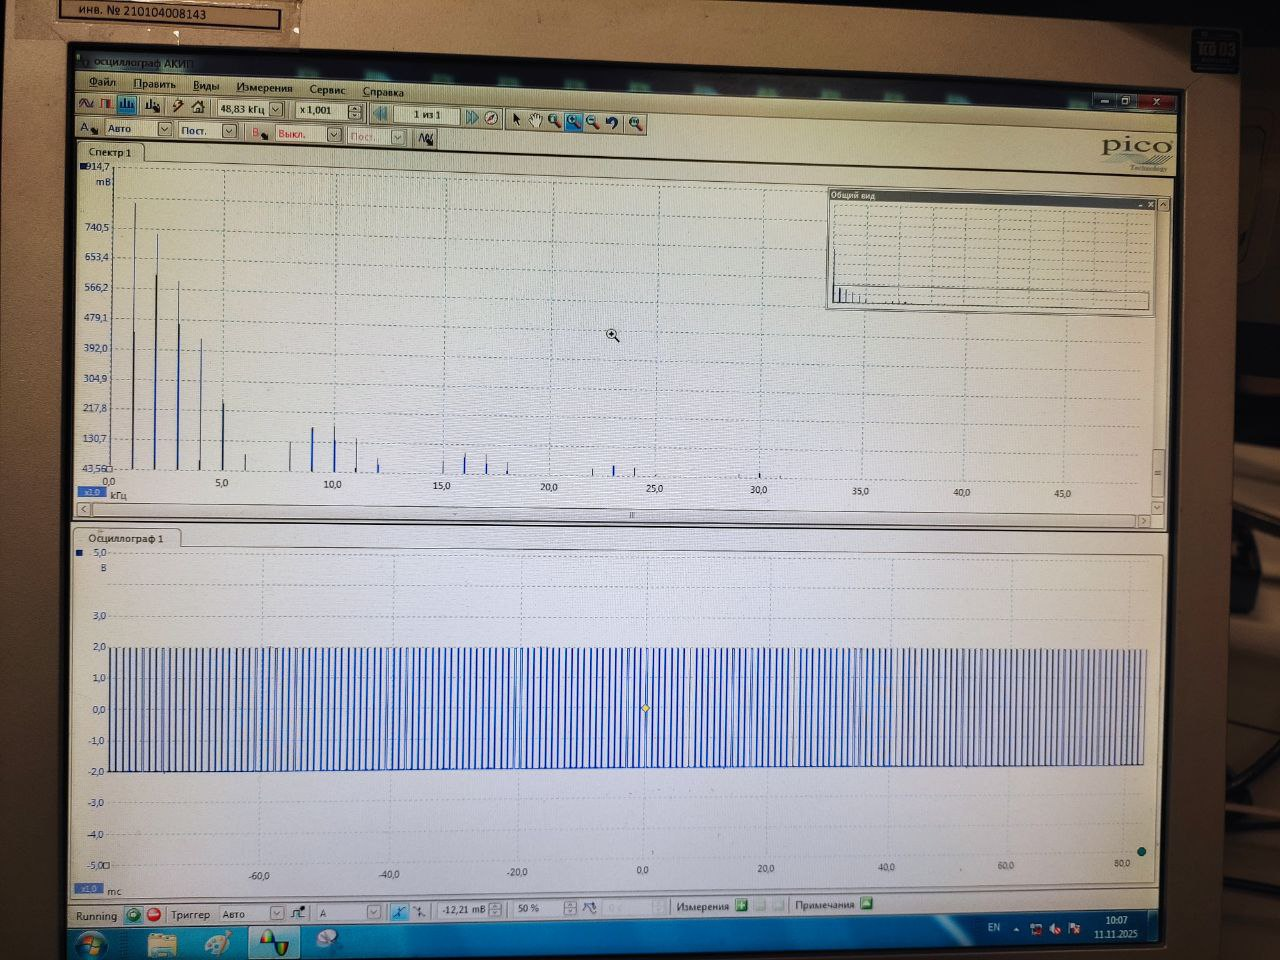
\includegraphics[width=10 cm]{100_1k.jpg}
        \caption{при изменении $\tau = 100 nsec$ при фиксированном $\nu_{\text{повт}} = 1000 Hz$}
        \label{fig:image1}
    \end{minipage}\hfill
    \begin{minipage}{0.48\textwidth}
        \centering
        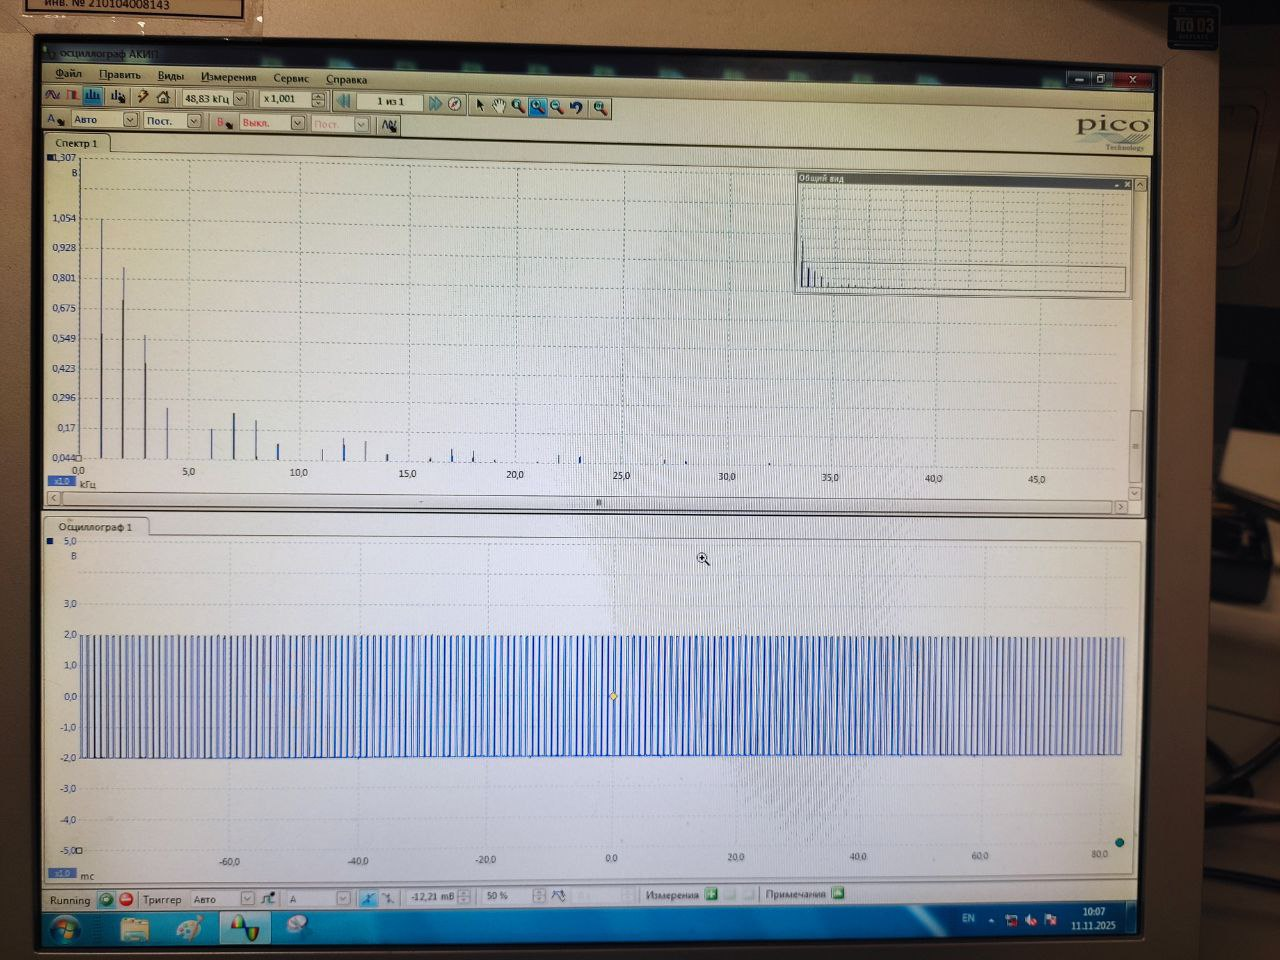
\includegraphics[width=10 cm]{150_1k.jpg}
        \caption{при изменении $\tau = 150 nsec$ при фиксированном $\nu_{\text{повт}} = 1000 Hz$}
        \label{fig:image2}
    \end{minipage}
\end{figure}

\newpage

\textbf{5.}Ознакомившись с методикой измерения параметров спектра , 
мы при фиксированных значениях $\nu_{\text{повт}} = 1000 Hz$ и $\tau = 50 mksec $  
измеряем амплитуды $a_n$ и частоты $\nu_n$ нескольких (6) спектральных компонент (гармоник).

\begin{table}[!h]
\centering
\begin{tabular}{|c|c|c|c|c|c|c|}
\hline
$n$ гармоники & 1 & 2 & 3 & 4 & 5 & 6 \\
\hline
$\nu_n^{\text{эксп}}$, кГц & 1.0 & 2.0 & 3.0 & 4.0 & 5.0 & 6.0 \\
\hline
$\nu_n^{\text{теор}}$, кГц & 1.0 & 2.0 & 3.0 & 4.0 & 5.0 & 6.0 \\
\hline
$|a_n|^{\text{эксп}}$, мВ & 290 & 278 & 272 & 263 & 256 & 242 \\
\hline
$|a_n/a_1|^{\text{эксп}}$ & 1.000 & 0.959 & 0.938 & 0.907 & 0.883 & 0.835 \\
\hline
$|a_n/a_1|^{\text{теор}}$ & 1.000 & 0.959 & 0.895 & 0.809 & 0.705 & 0.587 \\
\hline
\end{tabular}
\end{table}

$$\nu_n^\text{теор} = \frac{n}{T}$$
$$|a_n|_\text{теор} = \frac{|\text{sin}\frac{\pi n \tau}{T}|}{\pi n}$$


\newpage

\textbf{6.}Мы фиксируем период повторения $T = 1000 mcsec$ прямоугольного сигнала , $\nu_{\text{повт}} = 1~\text{кГц}$. 
Изменяя длительность импульса $\tau$ в диапазоне от $\tau = T/50$ до $\tau = T/5$, 
мы измеряем полную ширину спектра сигнала $\Delta\nu$ — от центра спектра ($\nu = 0$) до гармоники с нулевой амплитудой $a_n \approx 0$.

\begin{table}[h!]
    \centering
    \begin{tabular}{|c|c|c|c|c|c|c|c|c|}
\hline
$\tau$, мкс & 20 & 31 & 51 & 72 & 92 & 113 & 133 & 154 \\ \hline
$\Delta \nu$, кГц & 48,7 & 32,4 & 19,5 & 14 & 10,4 & 8,4 & 7,5 & 6,5 \\ \hline
$1/\tau \cdot 10^3$, с$^{-1}$ & 50 &  32,26& 19,61 &13,89  &10,87  &8,85  &7,52  &6,49 \\ \hline
\end{tabular}
\end{table}

Построим график зависимости  $\bigtriangleup \nu  (\frac{1}{\tau })$

\begin{figure}[h!]
	\centering
	
\includegraphics[width=19cm]{f1.PNG}
	\caption{график зависимости  $\bigtriangleup \nu  (\frac{1}{\tau })$}
	\label{fig:Holl2}
\end{figure}

\begin{enumerate}
    \item Уравнение прямой:
    \begin{equation}
    \Delta\nu = 0.247 + 0.987 \cdot (1/\tau \cdot 10^3),
    \label{eq:linear_fit_equation}
    \end{equation}

    \item Наклон прямой:
    \begin{equation}
    b = 0.987 \pm 0.015,
    \label{eq:slope_value_exp}
    \end{equation}

    \item Пересечение с осью $Y$:
    \begin{equation}
    a = 0.247 \pm 0.112,
    \label{eq:intercept_value}
    \end{equation}

    \item Наклон близок к 1, что указывает на пропорциональную зависимость $\Delta\nu \propto 1/\tau$.
        \item Небольшое отклонение от 1 и ненулевое пересечение объясняются погрешностями измерений.
        \item Погрешность наклона ($\pm 0.015$) рассчитана как стандартное отклонение коэффициента регрессии.
\end{enumerate}

\textbf{6.} Мы фиксируем длительность импульса прямоугольного сигнала (например, $\tau = 100~\text{мкс}$). 
Изменяя период повторения $T$ в диапазоне от $2\tau$ до $50\tau$, мы измеряем расстояние $\delta\nu = \nu_{n+1} - \nu_n$ между соседними гармониками спектра. 
Если спектральные компоненты окажутся расположенными слишком близко друг к другу, 
мы измеряем расстояние между $(n+m)$-й и $m$-й гармониками (для некоторых целых $n$ и $m$) и находим $\delta\nu = (\nu_{n+m} - \nu_n)/m$.

\centering
\begin{tabular}{|c|c|c|c|c|c|c|c|c|c|}
\hline
$T$, мкс & 200 & 600 & 1000 & 1400 & 1800 & 2200 & 3000 & 4000 & 5000 \\ \hline
$\delta \nu$, кГц & 10 & 1,65 & 1 & 0,72 & 0.56 & 0.46 & 0.34 & 0.27& 0.19 \\ \hline
\end{tabular}

\newpage

Построим график зависимости  $\delta \nu  (\frac{1}{T})$

\begin{figure}[h!]
	\centering
	
\includegraphics[width=19cm]{f2.PNG}
	\caption{график зависимости  $\bigtriangleup \nu  (\frac{1}{\tau })$}
	\label{fig:Holl2}
\end{figure}

Результаты линейной регрессии
\begin{enumerate}
\item Наклон прямой: $985.5 \pm 25.3$~кГц·период
Оценка погрешностей:
\item Относительная погрешность наклона: $\dfrac{25.3}{985.5} \times 100\% \approx 2.6\%$
    \item Это хороший результат для экспериментальных данных
\end{enumerate}    
\newpage
\subsection{Б. Наблюдение спектра периодической последовательности цугов}

\textbf{1} Следуя техническому описанию генератора, мы устанавливаем на нём режим подачи периодических импульсов синусоидальной формы. 
    Рекомендуемые параметры: частота несущей $v_0 = 50~\text{кГц}$, период повторения $T = 1~\text{мс}$ ($\nu_{\text{повт}} = 1~\text{кГц}$), 
    число периодов синусоиды в одном импульсе $N = 5$ (что соответствует длительности импульса $\tau = N / v_0 = 100~\text{мкс}$). 
    Мы получаем на экране осциллографа устойчивую картину сигнала.

	\begin{figure}[h!]
	\centering
	
\includegraphics[width=14cm]{p2.jpg}
	\caption{график зависимости  $\bigtriangleup \nu  (\frac{1}{\tau })$}
	\label{fig:Holl2}
	\end{figure}

\textbf{2} Мы получаем на экране осциллографа спектр сигнала. Центр картины мы устанавливаем на частоту $v_0$. 
    Масштаб по горизонтали (кГц/дел) мы подбираем так, чтобы спектр помещался на экране.

\textbf{3} Изменяя параметры сигнала $v_0$, $T$ и $N$, мы наблюдаем, как изменяется вид спектра. 
    Мы сравниваем наблюдаемые спектры со спектрами прямоугольных импульсов. 
Мы сохраняем или фотографируем несколько изображений спектров, подтверждающих результаты наблюдений. 

\centering
\begin{tabular}{|c|c|}
\hline
$\nu_{0} = 60 kHz$ & c = 60 kHz   \\ \hline
$T = 1 msec$ & $\bigtriangleup \nu = 24$ kHz   \\ \hline
N = 5& $\delta \nu = 1$ kHz   \\ \hline
\end{tabular}
\centering
\begin{tabular}{|c|c|}
\hline
$\nu_{0} = 50 kHz$ & c = 50 kHz   \\ \hline
$T = 10 msec$ & $\bigtriangleup \nu = 20$ kHz   \\ \hline
N = 5& $\delta \nu = 0,1$ kHz   \\ \hline
\end{tabular}
\centering
\begin{tabular}{|c|c|}
\hline
$\nu_{0} = 50 kHz$ & c = 50 kHz   \\ \hline
$T = 1 msec$ & $\bigtriangleup \nu = 10$ kHz   \\ \hline
N = 10& $\delta \nu = 1$ kHz   \\ \hline
\end{tabular}

\begin{figure}[H]
    \centering
    \begin{minipage}{0.48\textwidth}
        \centering
        \includegraphics[width=10 cm]{P14.jpg}
        \caption{До изменений}
        \label{fig:image1}
    \end{minipage}\hfill
    \begin{minipage}{0.48\textwidth}
        \centering
        \includegraphics[width=10 cm]{PN.jpg}
        \caption{при изменении $\nu$ (центр сместился с 50 до 60)}
        \label{fig:image2}
    \end{minipage}

    \centering
    \begin{minipage}{0.48\textwidth}
        \centering
        \includegraphics[width=10 cm]{P14.jpg}
        \caption{До изменений}
        \label{fig:image1}
    \end{minipage}\hfill
    \begin{minipage}{0.48\textwidth}
        \centering
        \includegraphics[width=10 cm]{Pt.jpg}
        \caption{при изменении $T$}
        \label{fig:image2}
    \end{minipage}

    \centering
    \begin{minipage}{0.48\textwidth}
        \centering
        \includegraphics[width=10 cm]{P14.jpg}
        \caption{До изменений}
        \label{fig:image1}
    \end{minipage}\hfill
    \begin{minipage}{0.48\textwidth}
        \centering
        \includegraphics[width=10 cm]{Pnn.jpg}
        \caption{при изменении $N$}
        \label{fig:image2}
    \end{minipage}
\end{figure}

\newpage

\subsection{Г. Исследование спектра амплитудно-модулированного сигнала}

\begin{enumerate}
    \item[\textbf{1}] Следуя техническому описанию генератора, мы устанавливаем на нём режим модулированного по амплитуде синусоидального сигнала. 
    Рекомендуемые параметры: частота несущей $v_0 = 50~\text{кГц}$, частота модуляции $\nu_{\text{мод}} = 2~\text{кГц}$, глубина модуляции $50\%$ ($m = 0{,}5$). 

    \item[\textbf{2}] С помощью осциллографа (в режиме курсорных измерений) мы измеряем максимальную $A_{\max} = 1,25 B$ и минимальную $A_{\min} = 415 mB$ амплитуды сигнала. 
    Мы убеждаемся в справедливости равенства $m = \dfrac{A_{\max} - A_{\min}}{A_{\max} + A_{\min}} = 0,5$.

    \item[\textbf{3}] Мы получаем на экране спектр сигнала. С помощью осциллографа (в режиме курсорных измерений) мы измеряем частоты центральной $\nu_{\text{центр}} = 50 kHz$ и боковых гармоник  $\nu_{\text{бок}} = 52 kHz$. 
    Изменяя несущую частоту $v_0$ и частоту модуляции $\nu_{\text{мод}}$, мы наблюдаем, как изменяется положение спектральных линий. 

    \item[\textbf{4}] Изменяя на генераторе глубину модуляции $m$ в диапазоне от $10\%$ до $100\%$ (всего 7 точек), 
    мы измеряем отношение амплитуд боковой и основной спектральных линий $\dfrac{a_{\text{бок}}}{a_{\text{осн}}}$.

\end{enumerate}

\begin{center}
\begin{tabular}{|c|c|c|c|c|c|c|c|}
\hline
$m$, \% & 10 & 25 & 40 & 55 & 70 & 85 & 100 \\ \hline
$a_{\text{бок}}$, мВ & 29 & 72 & 117 & 160 & 203 & 247 & 295 \\ \hline
\multicolumn{8}{|c|}{$a_{\text{осн}}$ = 586 мВ} \\ \hline
$a_{\text{бок}}/a_{\text{осн}}$ & 0.0495 &0.1229  &0.1997  & 0.2730 & 	
0.3464 & 0.4215 &0.5034 \\ \hline
\end{tabular}
\end{center}

Построим график зависимости $\frac{a_{\text{бок}}}{a_{\text{осн}}}(m)$

	\begin{figure}[h!]
	\centering
	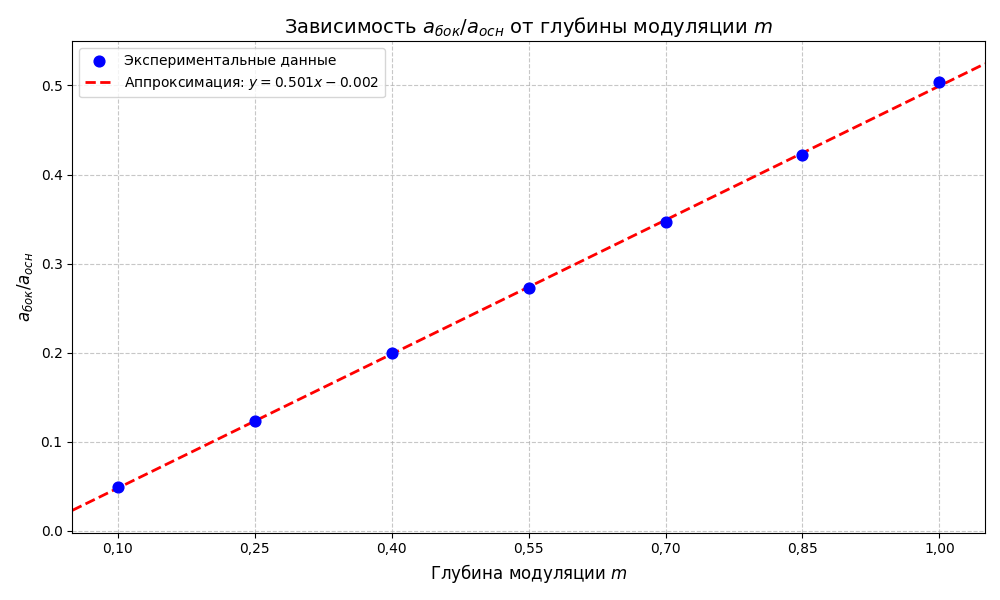
\includegraphics[width=18cm]{F3.png}
	\caption{график зависимости $\frac{a_{\text{бок}}}{a_{\text{осн}}}(m)$}
	\label{fig:Holl2}
	\end{figure}


Используя МНК, получим $k=0.5014x\pm0,001$, что подтверждает $\frac{a_{\text{бок}}}{a_{\text{осн}}}=\frac{m}{2}$, т.е. совпадает с теоретическим предсказанием. График приведён на рис. 20.

\newpage

\subsection{Е. Изучение фильтрации сигналов}

\begin{figure}[h!]
	\centering
	
\includegraphics[width=10cm]{p6.png}
	\caption{ Схема экспериментальной установки для изучения фильтрации сигналов }
	\label{fig:Holl2}
\end{figure}

\begin{enumerate}
    \item[\textbf{1}] Для $RC$-цепочки ($RC$-фильтр низких частот) с известными сопротивлением и ёмкостью мы рассчитываем её характерное время $\tau_{RC} = RC = 3 mcSec$ 
    и соответствующую частоту $\nu_{RC} = 1 / \tau_{RC} = 0.3333 MHz$. Мы собираем схему согласно рис.21. 
    На вход $RC$-цепочки мы подаём последовательность прямоугольных импульсов с периодом повторения $T \sim \tau_{RC}$ и длительностью $\tau \sim T/20$.

    \item[\textbf{2}] Мы наблюдаем форму сигнала и его спектр на выходе $RC$-цепочки («фильтрованный» сигнал) при различных значениях периода повторения $T$. 
    
    \item[\textbf{3}] При некотором фиксированном периоде $T$ мы проводим измерения отношений амплитуд соответствующих спектральных гармоник 
    (для 7 гармоник) фильтрованного и исходного сигналов: $K_n = |a_n^{\text{ф}}| / |a_n^{0}|$. 
    Чтобы измерить амплитуды $a_n^{0}$ спектра исходного сигнала, мы переподключаем генератор к первому каналу осциллографа напрямую 
    или с помощью отдельного кабеля подаём нефильтрованный сигнал на второй канал осциллографа.

\end{enumerate}

    \centering
    \begin{tabular}{|c|c|c|c|c|c|c|c|}
    \hline
        $a_{n}^{\text{Ф}}$ mB& 96 & 46 & 33 & 24 & 18 & 15& 10  \\ \hline
        $a_{n}^{\text{0}}$ mB& 232 & 232 & 229 & 223 & 218 &  211& 201 \\ \hline
		$K_n$ & 0.4138 &0.1983  &0.1441  &0.1076  & 	
0.0826 &0.0711  &0.0498 \\ \hline
    \end{tabular}

Построим график зависимости  амплитудного коэффициента фильтрации $K_{\nu}$ от частоты $\nu$

\begin{figure}[h!]
	\centering
	\includegraphics[width=19cm]{f4.png}
	\caption{ график зависимости  амплитудного коэффициента фильтрации $K_{\frac{1}{\nu}}$ от частоты $\nu$ }
	\label{fig:Holl2}
\end{figure}

Из коэффициента наклона получаем $\tau_{RC} = (3.3 \pm 0.2)мкс$


\newpage

\section{Выводы}
Изучили спектры сигналов различной формы и влияние параметров сигнала на вид соответствующих спектров; проверили справедливость соотношений неопределённостей; познакомились с работой спектральных фильтров на примере RC-цепочки. 
Проверили выполнение физических законов и моделей в реальных условиях. Все они выполнились с высокой точностью. 

\end{document}